\section{Data Requirements}\label{sec:data_requirements}
The information that is required to setup and run an age based model in \CNAME, but is by no means the end all and be all (because you can add in any functionality you wish). An age based model refers to how \CNAME\ keeps track of the population, this is by keeping track of the numbers at age for each category in the population.
\begin{enumerate}
	\item Catch History (currently \CNAME\ assumes this is known without error)
	\item Time series of relative/absolute abundance/biomass
	\item Age/length compositional data (if you want to estimate selectivities or year class strengths)
	\item Some recruitment process
	\item Biological information (e.g. growth, maturity, life cycle)
\end{enumerate}
In theory recruitment and biological information is all that is needed to run a \CNAME\ model, obviously that would not include any anthropogenic exlpoitation processes and so can be thought of as a equilibrium or steady-state model.

The biological information that would be required will depend on if you are going to need to do weight calculations. For an age based model you will need to specify 
\begin{enumerate}
	\item length at age \command{age\_length}
	\item weight at length \command{length\_weight}
	\item natural mortality \command{process}	
\end{enumerate}

\begin{figure}[htp]
			 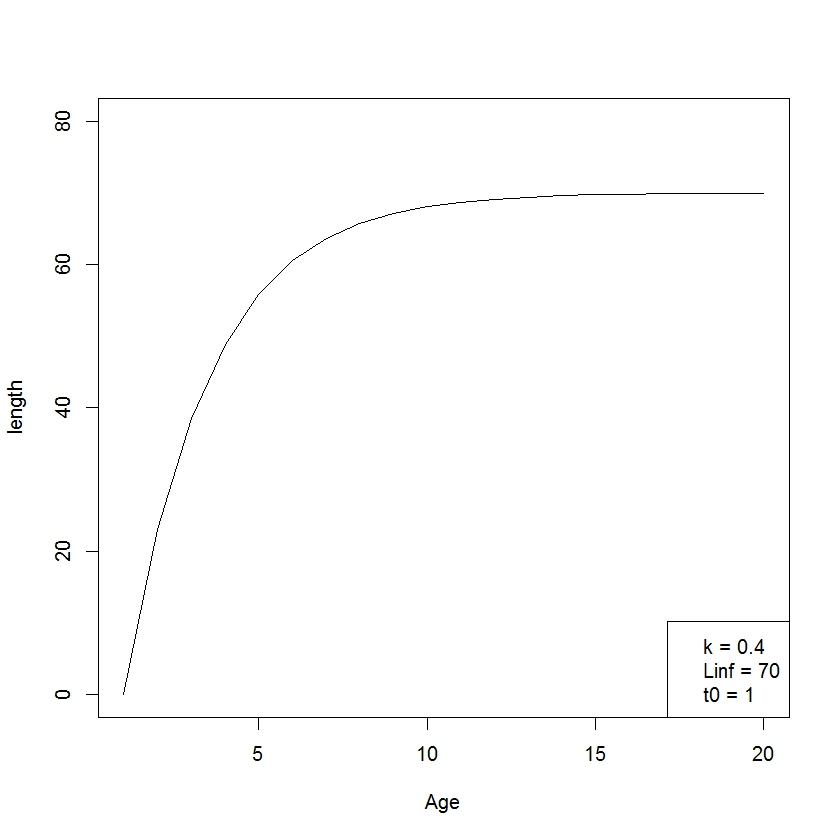
\includegraphics[scale=0.4]{Figures/VonBert.jpeg}
			 \caption{\textbf{An example of a Von Bertalanfy growth curve.}}
\end{figure}



